\documentclass[man,natbib]{apa6}

\title{Personal statement on learning and instruction}
\shorttitle{Learning and instruction}
\author{Colby Goettel}
\affiliation{Brigham Young University}

\usepackage{graphicx}

\newcommand\vref[3]{(#1~#2\thinspace:\thinspace#3)}

\abstract{David Kolb defined learning as ``the process whereby knowledge is created through the transformation of experience'' \citep{kolb2014experiential}. Learning is an experienced activity. Knowledge can be carried to the learner, but the learner must choose to work and rework that knowledge until it has become a part of them. This internalization is how knowledge is created: the learner must construct it once it has been brought to them. Simply transmitting knowledge is not enough to cause learning to happen.}

\begin{document}
\maketitle

% The purpose of learning
The purpose of learning is to grow as an individual. To grow as a society. To better mankind. Everything we do, or everything we ought to do, is to better mankind. As a student, my purpose for learning is to better mankind. There's a reason BYU's motto ends ``go forth to serve.'' As a disciple, my purpose is to ``first seek to obtain [the Lord's] word'' \vref{D\&C}{11}{21}~--- to learn~--- and \emph{then} to apply it and better myself and better mankind.

Even as a Linux system administrator, my purpose is to better mankind. This is why open source software and documentation are so important: the one is able to benefit the many. For information technology (IT) professionals, everything we need to know is online. We built the Internet and put everything we know on it. At this point, there will probably only be one or two problems in my career that no one else has already encountered and documented. And when I encounter those problems, I will document them and make them easy to find. I've already encountered one such problem and I immediately wrote a post about it. And several months later when I needed the same answer, I Googled it and found my previous post. This is how we better mankind.

Learning is to be shared. Maybe not the experience and process of learning, but once learning has been internalized and become knowledge, that is to be shared.

% The intended goals of instruction
This dissemination of knowledge~--- instruction~--- is central to the purpose of learning. What's the point of learning something if no one else is benefited by it? This even holds up theologically. I believe the Lord (as always) has shown us the correct example here: when the Lord teaches us something, we should be responsible stewards and write it down; the Lord should never have to tell us something more than once. His instructions are to be recorded and referenced, not rejected and re-sought.

% Your position regarding the process of learning and instruction. For example, your assumptions about the roles and responsibilities of teachers and learners, what your approach values and emphasizes, the techniques you'd be inclined to use, the ideal outcomes of learning, etc. (brief examples or narratives may help).
\section{Where I stand}
My sophomore year in high school (2003), we took the Myers-Briggs Type Indicator (MBTI). It nailed me to a T. This early experience helped solidify cognitivism as a credible theory because of its incredible accuracy. As I've aged and my MBTI results have changed,\footnote{From INFP to INTJ.} the test has continued to stand true for who I am now.

Behaviorism and cognitivism make so much sense to me because they both have an emphasis on hard, scientific results. Everything in IT is based on hard facts. During my literature review for my prospectus, every single article I read was a quantitative study. It was astounding that there was no mixed method or qualitative. But it's understandable because when technical people read an article and it talks about how certain something is, we want a $p$-value. We want to see \emph{exactly} how strong the correlation is. None of this wishy-washy thinking that is so often found in the softer sciences. We're used to working with computers: you tell a computer what to do and it does exactly that. Nothing more, nothing less. Why should research be any different? Give me the facts. Show me the money.

Constructivism also provides an enticing avenue because everything must be learned. Going to class and being told things isn't enough. In IT, we have labs attached to almost every class because without the application, the theory is never learned. Every idea that is transmitted needs to be constructed in the mind of the learner for true learning to happen.

While I recognize that situated learning and narrative are valid and (at least partially) true, they don't work in my field. We don't do much ethnographic research in IT. And there's no phenomenology; it just doesn't make sense in technology.

In the movie \textit{Donnie Darko}, one of Donnie's teachers, Kitty Farmer, is teaching the class about the ``lifeline,'' a spectrum ranging from fear to love. She tries to have Donnie simplify a scenario onto the lifeline, but Donnie freaks out, stating ``[y]ou can't just lump everything into these two categories and then just deny everything else.'' ``[T]he whole spectrum of human emotion'' cannot be simplified into a two-dimensional spectrum: life is too complex to split into two camps. While it might seem that cognitivism and behaviorism are too narrow and simplistic to truly cover the gambit of human emotion and thinking, they work for so many use cases that they're worthwhile.

Finally, I'm wary of any theory that is referred to as ``esoteric.'' Nothing in this field has been difficult to understand except for the poor writing. But poor writing aside, all of the theories, even the softer ones, have been completely easy to understand. If something is esoteric, it's probably just wrong. See Figure~\ref{fig:science-articles-writing}.
\begin{figure}[h]
    \centering
    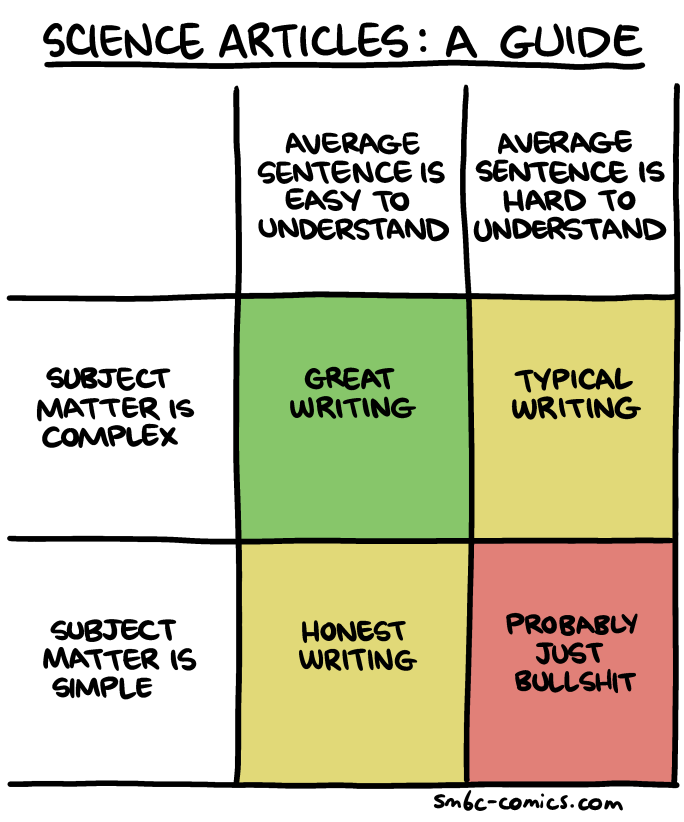
\includegraphics[width=0.55\textwidth]{science-articles-writing}
    \caption{Mouse-over text: ``All philosophy comics are off the chart, down and to the right.'' \citep{smbc}}
    \label{fig:science-articles-writing}
\end{figure}

% Core theoretical ideas that make up your viewpoint. Includes: meaning of key concepts such as agency, learning, teaching, instruction, technology, skill, knowledge, etc.
\section{David Kolb's experiential learning theory}
I'm pretty sold on the experiential learning theory (ELT) that David Kolb has propagated \citep{kolb2005kolb} and used as the basis for his learning styles inventory (LSI). This theory has its roots in Dewey, Lewin, Piaget, William James, Jung, Freire, Carl Rogers, and others.\footnote{A quick side note on combining theories: I know that people freak out when we take different people's opinions and mash them together, but I think that's childish. There's so much overlap in these theories that it just makes sense to take a little from one and another little from another. This isn't theology, we're allowed to use other people's ideas as we see fit.}

Some key points from Kolb's ELT are discussed in the following subsections.
\subsection{Learning is a process}
``Learning is best conceived as a process, not in terms of outcomes.'' I love this. Yes, I do care about the outcome, but I really care about the journey. It's all about the journey because that's how you get places. People definitely differ on this, but I've always cared more about the methodology and the findings than the conclusion.

\subsection{All learning is relearning}
``All learning is relearning.'' We must constantly be retaught things in order to truly learn them. There's a big reason the Lord repeats so often.

\subsection{Conflict drives learning}
``Conflict, differences, and disagreement are what drive the learning process.'' The times in my life that I have learned the most have come from having to argue something out. My best prayers have been when I've come into my room, closed my door, and said out loud, ``Okay, we need to talk about this.'' These prayers have taken up to an hour before as I've hashed things out with the Lord and come to a proper understanding of things.

\subsection{Process of creating knowledge}
``Learning is the process of creating knowledge.'' This is focusing on what I think is a semantic difference that we all just need to get over. This view is based on constructivism which says that a learner constructs new knowledge: ``social knowledge is created and recreated in the personal knowledge of the learner.'' It's contrasted to the transmission model whereby ``pre-existing fixed ideas are transmitted to the learner.'' This is purely semantic in my brain. Maybe I'm just too technical and not philosophical enough (or whatever), but if knowledge is transmitted to the learner, the learner still has to construct that knowledge in their brain. I see learning like a child being given a new Lego set for Christmas: the Lego set is ``transmitted'' to the child, but the child must then ``construct'' the set into a final product. Constructing the product is what learning is all about. Mistakes will be made. The child might even have to rebuild the set a few times to really get it down. To carry this another step further, once the child has finished this set (learned new concepts), they must then deconstruct and reconstruct their previous knowledge to fit into this new paradigm.

It's like learning to play the piano. My piano teacher growing up would always ask me if I had played or if I had practiced. I always said that I'd practiced because that's what I called it when I sat at the piano and played things. However, there was an important distinction she was trying to emphasizing: ``playing'' is sitting down and playing through the song; ``practicing'' is going through a song and, when a struggle point is reached, playing it over and over again until it's no longer a struggle.

Much like the child building a Lego set, it's important to find weak points in the learning process and go over them again and again until the set or piece is completed.

\section{Conclusion}
Were I ever asked to define learning (as I am in this paper), I would directly quote David Kolb: Learning is ``the process whereby knowledge is created through the transformation of experience'' \citep{kolb2014experiential}. Humans have experiences. These experiences, once internalized (transformed), become knowledge. This is the whole of learning. There are many additional theories that attempt to define how humans think and act, but as far as learning goes, it is the creating of knowledge by having experiences, pondering those experiences, coming to conclusions, and storing that information.

% References from the scholarly literature (including from class) to situate your viewpoint in the world of ideas and help support your claims.
\bibliography{references}

\end{document}

Usually has the following features:
- Clearly identified audience/context at the beginning
- Modest scope: don't try to take on too much (less is more)
- Important assertions clarified and supported
- Smooth flow, coherent organization. Often with section headings.
